\documentclass[11pt, a4paperm, hidelinks]{article}
\usepackage[utf8]{inputenc}
\usepackage[T1]{fontenc}
\usepackage[english]{babel}
\usepackage{lmodern}


\usepackage[a4paper,top=3cm,bottom=3cm,left=3cm,right=3cm]{geometry}
\usepackage{chngcntr}

%package used to enumerate figures
\usepackage[labelfont=bf]{caption}

%hyperref for interactive PDF index
\usepackage[bookmarks, colorlinks, breaklinks]{hyperref}
\hypersetup{linkcolor=black, citecolor=black, filecolor=black, urlcolor=black}

%Package required to use special symbols
\usepackage{amsmath, amssymb}

%Package required to use figures
\usepackage{graphicx}
\usepackage{subfig}
\usepackage{placeins}

%Include the bibliography in the table of contents
\usepackage{tocbibind}

%Package used to insert figures at the specified position
\usepackage{float}
\usepackage{longtable}

\usepackage{times}

%Our chapters must be called sections
\addto\captionsenglish{\renewcommand{\chaptername}{Section}}

%Header
\usepackage{fancyhdr}
\pagestyle{fancy}
\fancyhf{}
\rhead{Stefano Bagarin - Alessandra Pasini}
\lhead{Usability Evaluation Study 1: Inspection}
\rfoot{Page \thepage}

\begin{document}

	%Code for title page
	\begin{titlepage}
		\centering
		
\includegraphics[width=0.20\textwidth]{./assets/polimi-logo.png}\par

		{Politecnico di Milano \\ AA 2019/2020} \par
		\vspace{1.5cm}

		{Computer Science and Engineering}\par
		\Large{Hypermidia Applications}\par
		\vspace{1.0cm}

		{\LARGE \textbf{Usability Evaluation Study 1: Inspection} \par}
		\vspace{1.5cm}

		{\normalsize {\textbf{Stefano Bagarin}: mrt. 945159 -  stefano.bagarin@mail.polimi.it }\par}
		\vspace{0.2cm}
		{\normalsize{\textbf{Alessandra Pasini}: mtr. 920051 - alessandra.pasini@mail.polimi.it}\par}
		\vspace{1.0cm}
		
		{\normalsize {\textbf{Inspected website}: \url{https://www.visitmonterosa.com/}}\par}
		\vspace{0.2cm}
		{\normalsize {\textbf{Delivery Date}: }\par}
		\vfill

		% Bottom of the page
		{\large Document version: 1.0\par}
		{\large \today \par}
	\end{titlepage}

	%Make the table of contents
	\tableofcontents
	\clearpage


	%Abstract
	%\chapter{Abstract}
	%\label{ch:Abstract}
	\section{Abstract}
	The aim of this document is to report the Inspection-based Usability Evaluation of \emph{Visit Monterosa} website which can be found at the following url \url{https://www.visitmonterosa.com/}. \\ TODO: The analysed website provides extensive
information about the Natural Park of Adamello – Brenta including descriptions of local history
and environment, activities and attractions available in the park paired with an interactive map of
tracks, initiatives organized by the park authorities and much more. The contents include an
analysis on through heuristic inspection of XX expert evaluators and an overall evaluation of the
product along with our conclusions. The Annex provides the individual scores of each inspector.


goal 1 : trovare esperienze e pronarle   “Searching information about experiences and opportunities”
goal 2 : prenotare vacanza 
goal 3 : avere informazioni sul monterosa
	\clearpage


	%Inspection Methods
	%\chapter{Inspection Methods}
	%\label{ch: Inspection Methods}
	\section{Inspection Methods}

	\subsection{Overview}
	The inspection process started with the definition of both heuristics and score metrics, after a deep understanding of those concepts; then it went trough the choice of the main goals to have in mind while analyzing the website; the indivitual scoring and the final evaluation given by the average of individual ratings.\\
The following sections have the aim to highlight some of the steps taken during the inspection process and underline some foundamental concepts necessary to understand the final result.

	\subsection{Heuristic}
	The used heuristics can be divided into three cateogries depending on their final purposes and goals. Here is possible to find the groups definitions and the heuristics in each of them: \\ 
\\
\textbf{Navigation:} this batch has the aim to evaluate how easy is to move across the website and how easy and intuitive is to find contents following the websites paths.
	\begin{itemize}
		\item \textbf{Interaction consistency:} do pages of the same type have the same links and interaction capability?
		\item \textbf{Group navigation:} is it easy to navigate among group members and from a group introductory page to 				group members (and the other way around)?
		\item \textbf{Structural Navigation:} is it easy to navigate among the semantic components of a Topic?
		\item \textbf{Semantic Navigation:} is it easy to navigate from a Topic to a related one?
		\item \textbf{Landmarks:} are landmarks useful to reach the key parts of the web site?
	\end{itemize}
\textbf{Contents:} focuses on the quality of information and data provided by the site regardless the way they are presented. 
	\begin{itemize}
		\item \textbf{Information Overload:} is the information in a page too much or too little and does it fit the page layout?
		\item \textbf{Quality of Contents:} do the contents of the page include the informations that the user should expect 				there? In other words, is the content consistent.
	\end{itemize}
\textbf{Layout:} stresses the visual image of the website and its effectiveness in terms of expressivity and ergonomic functions. 
	\begin{itemize}
		\item \textbf{Text Layout:} is the text readable? Is font size appropriate?
		\item \textbf{Interaction Placeholder:} are textual or visual labels of interactive elements “expressive”? i.e., do they reflect 			the meaning of the interaction and its effects? Are they consistent?
		\item \textbf{Spatial Allocation:} is the on-screen allocation of contents and visual appropriate for their relevance? Are 				“semantically related” elements close and “semantically distant” element far away?
		\item \textbf{Consistency of Page Structure:} do pages of the same type have the same lay out (same visual properties of 			each component and similar lay-out organization of the various elements?) 
	\end{itemize}


	\subsection{Scoring Metrics}
	In order to evaluate every heuristic defined in the previous section, it has been choosen a scoring system with votes between 0 and 5. The following figure shows the meaning of each scores. 
\begin{figure}[h!]
	\centering
 	\begin{minipage}[b]{1\textwidth}
    		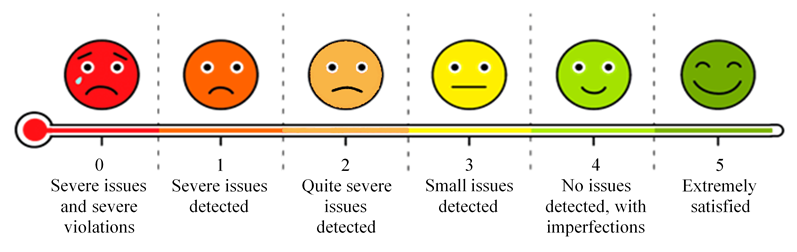
\includegraphics[width=\textwidth]{./assets/scoring.png}
	\end{minipage}
\end{figure}
\FloatBarrier

	\subsection{Goals}
	Before starting the process, the following goals have been defined to better inspect the website and to work in a more precise way.
\begin{itemize}
	\item \textbf{Goal 1:} Find experiences' information and book them
	\item \textbf{Goal 2:} Book an holiday
	\item \textbf{Goal 3:} Searching info about Monte Rosa

\end{itemize}

	\subsection{Final Evaluation}
Verrà analizzato nel capito dopo
Introduzione dicendo che i valori sono ottenuti secondo la metrica scelta dai valori individuali che si trovano nell’appendice


	\subsection{Report}



	%Agreed scores on each individual heuristics
	%\chapter{Agreed scores on each individual heuristics}
	%\label{ch: Agreed scores on each individual heuristics}
	\section{Agreed scores on each individual heuristics}

	\subsection{Navigation}

	\subsection{Content}

	\subsection{Layout}


	%Aggregated Results and Discussion
	%\chapter{Aggregated Results and Discussion}
	%\label{ch: Aggregated Results and Discussion}
	\section{Aggregated Results and Discussion}
Con charts tipo lavoro


	%Conclusions
	%\chapter{Conclusions}
	%\label{ch:Conclusions}
	\section{Conclustion}


	%Appendix
	\appendix
	%\chapter{Appendix}

\end{document}
